% !TEX TS-program = pdflatex
% !TEX encoding = UTF-8 Unicode
% This file is a template using the "beamer" package to create slides for a talk or presentation
% - Talk at a conference/colloquium.
% - Talk length is about 20min.
% - Style is ornate.
% - Trial 
% MODIFIED by Krishna Kumar, 2011
% The header comments and encoding in this file were modified for inclusion with TeXworks.
% The content is otherwise unchanged from the original distributed with the beamer package.

 \documentclass[10pt,xcolor=table]{beamer}


% In principle, this file can be redistributed and/or modified under
% the terms of the GNU Public License, version 2.


\mode<presentation>
{
  \usetheme{Madrid}
  % or ...

  \setbeamercovered{transparent}
  % or whatever (possibly just delete it)
}


\usepackage[english]{babel}
\usepackage[utf8]{inputenc}
\usepackage{textcomp}
\usepackage{caption}
\captionsetup{font=scriptsize, labelfont=scriptsize, justification=centering} % labelformat=empty} %,labelsep=none,}
\usepackage{times}
\usepackage{graphicx}
\usepackage{amssymb}
\usepackage[T1]{fontenc}
\usepackage{amsmath}
\usepackage{multirow}

% Note that the encoding and the font should match. If T1
% does not look nice, try deleting the line with the fontenc.


\title [\LaTeX for Beginners]
{A not so short introduction to \LaTeX2e \\ $\backslash$begin\{document\}\dots}
%\subtitle
%{Include Only If Paper Has a Subtitle}

\author[Krishna Kumar] % (optional, use only with lots of authors)
{Krishna Kumar \inst{*}\thanks{kks32@cam.ac.uk}\\ } % \and S.~Another\inst{2}}
% - Give the names in the same order as the appear in the paper.
% - Use the \inst{?} command only if the authors have different
%   affiliation.

%\pgfdeclareimage[height=0.2cm]{uni}{Cam.pdf}
%\logo{\pgfuseimage{uni}}
\institute[ University of Cambridge ] % (optional, but mostly needed)
{
  \inst{1}%
%  \and
%  \inst{2}%
King's College\\ University of Cambridge}
% - Use the \inst command only if there are several affiliations.
% - Keep it simple, no one is interested in your street address.
\date[King's Computing Workshop 2013] % (optional, should be abbreviation of conference name)
{King's Computing Workshop, October 2013}
% - Either use conference name or its abbreviation.
% - Not really informative to the audience, more for people (including
%   yourself) who are reading the slides online

\pgfdeclareimage[height=0.5cm]{university-logo}{figs/Engineering.png}
 %\logo{\pgfuseimage{university-logo}}

% If you have a file called "university-logo-filename.xxx", where xxx
% is a graphic format that can be processed by latex or pdflatex,
% resp., then you can add a logo as follows:

% Delete this, if you do not want the table of contents to pop up at
% the beginning of each subsection:
\AtBeginSubsection[]
{
  \begin{frame}<beamer>{Outline}
    \tableofcontents[currentsection,currentsubsection]
  \end{frame}
}


% If you wish to uncover everything in a step-wise fashion, uncomment
% the following command: 

%\beamerdefaultoverlayspecification{<+->}

\begin{document}
\begin{frame}
  \titlepage
\end{frame}

%**********************************************INTRODUCTION***************************************
\section{Introduction to \LaTeX2e}
%**********************************************FRAME***************************************
\begin{frame}
\frametitle{Developers}
\begin{itemize}
\item
\parbox{0.25\textwidth}{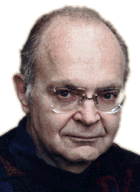
\includegraphics[width=0.15\textwidth]{figs/Donald_Knuth.png}}\hspace{0cm}
\parbox{0.65\textwidth}{Donald Knuth, 1977, \TeX ~Version 3.141592}
\item
\parbox{0.25\textwidth}{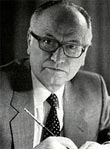
\includegraphics[width=0.15\textwidth]{figs/Hermann.jpg}}\hspace{0cm}
\parbox{0.65\textwidth}{Hermann Zapf}
\item
\parbox{0.25\textwidth}{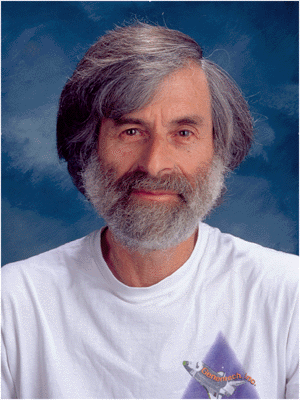
\includegraphics[width=0.15\textwidth]{figs/Leslie.png}}\hspace{0cm}
\parbox{0.65\textwidth}{Leslie Lamport, \LaTeX2e}
\end{itemize}
\end{frame}

%**********************************************INTRODUCTION***************************************
\section{Structure}
%**********************************************FRAME***************************************
\begin{frame}{LaTeX Structure}
\begin{figure}
\centering
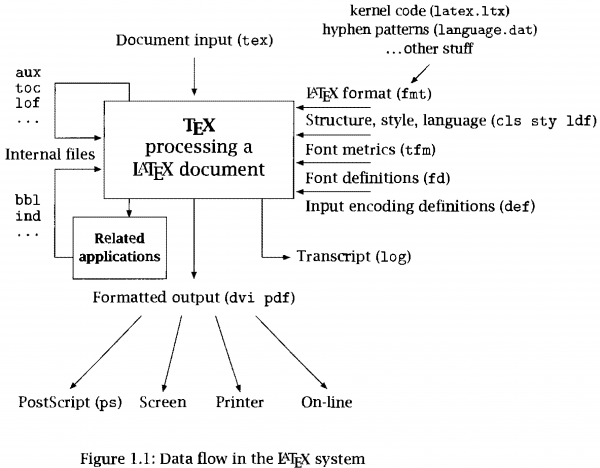
\includegraphics[width=0.7\textwidth]{figs/LaTeX.png}
\end{figure}
\end{frame}


%**********************************************FRAME***************************************
\begin{frame}{$\backslash$documentclass\{\}}

\begin{table}
\rowcolors{1}{pink}{white}
\begin{tabular}{|l|p{0.75\textwidth}|}
\hline
article & articles in scientific journals, presentations, short reports, program documentation, invitations, \dots \\ \hline
IEEEtran & IEEE Transactions format.\\ \hline
proc & A class for proceedings based on the article class.\\ \hline
minimal & Is as small as it can get. It only sets a page size and a base font. It is mainly used for debugging purposes.\\ \hline
report & For longer reports containing several chapters, small books, thesis, \dots \\ \hline
book & For real books.\\ \hline
slides & For slides. The class uses big sans serif letters.\\ \hline
memoir & For changing sensibly the output of the document. It is based on the book class, but you can create any kind of document with it\\ \hline
letter & For writing letters. \\ \hline
beamer& For writing presentations \\ \hline
\end{tabular}
\end{table}
\end{frame}


%**********************************************FRAME***************************************
\begin{frame}{Article, Report and Book}
\begin{table}
\begin{tabular}{|l|c|l|c|}
\hline
\multicolumn{2}{c}{\textbf{Article}}  & \multicolumn{2}{c}{\textbf{report}} \\ 
\hline
\textbf{section} &\textbf{ numbering} & \textbf{section} & \textbf{numbering} \\ \hline
$\backslash$part & 0 & $\backslash$part & -1 \\ \hline
$\backslash$chapter & 0 & $\backslash$section & 1 \\ \hline
$\backslash$section & 1 & $\backslash$subsection & 2 \\ \hline
$\backslash$subsection & 2 & $\backslash$subsubsection & 3 \\ \hline
$\backslash$subsubsection & 3 & $\backslash$paragraph & 4 \\ \hline
$\backslash$paragraph & 4 & $\backslash$subparagraph & 5 \\ \hline
$\backslash$subparagraph & 5 & & \\ \hline

\end{tabular}
\end{table}
\end{frame}

%**********************************************FRAME***************************************
\begin{frame}{$\backslash$documentclass$[$\textbf{options}$]$\{\}}
\begin{table}
\rowcolors{1}{white}{green}
\begin{tabular}{|p{0.15\textwidth}|p{0.65\textwidth}|}
\hline
Xpt & Sets the size of the main font in the document. Default: 10pt. \\
a4paper, \newline letterpaper & Defines the paper size. Default: letter/A4. \\
fleqn & displays formulas left-aligned instead of centered. \\
leqno & Places the numbering of formulas on the left hand side instead of the right. \\
titlepage,\newline  notitlepage & Specifies whether a new page should be started after the document title or not. The article class does not start a new page by default, while report and book do.\\
onecolumn,\newline  twocolumn & Instructs LaTeX to typeset the document in one column or two columns. \\
\end{tabular}
\end{table}
\end{frame}


%**********************************************FRAME***************************************

\begin{frame}{$\backslash$documentclass$[$\textbf{options}$]$\{\} cont \dots}
\begin{table}
\rowcolors{1}{white}{green}
\begin{tabular}{|p{0.15\textwidth}|p{0.65\textwidth}|}
twoside,\newline  oneside & double or single sided output. Article and report are single sided and the book is double sided by default. \\
landscape & Changes the layout of the document to print in landscape mode. \\
openright,\newline  openany & Makes chapters begin either only on right hand pages or on the next page available. This does not work with the article class, as it does not know about chapters. \\
draft & Draft - no images. \\
\end{tabular}
\end{table}
\end{frame}



%**********************************************FRAME***************************************

\begin{frame}{Restricted Characters}
\begin{table}
\begin{tabular}{cc}
\hline
\textbf{Character} & \textbf{How to type in LaTeX} \\  \hline
\# & $\backslash$\# \\ 
\& & $\backslash$\& \\ 
\$ & $\backslash$\$ \\
\% & $\backslash$\% \\ 
$\backslash$ & \$$\backslash$backslash\$ \\ 
\_ & $\backslash$\_ \\
\{ & $\backslash$\{ \\
\} & $\backslash$\} \\

\end{tabular}
\end{table}
\end{frame}


%**********************************************FRAME***************************************
\begin{frame}{Fonts}
\begin{itemize}
\item \tiny $\backslash$tiny
\item \scriptsize $\backslash$scriptsize
\item \footnotesize $\backslash$footnotesize
\item \small $\backslash$small
\item \normalsize $\backslash$normalsize
\item \large $\backslash$large
\item \Large $\backslash$Large
\item \LARGE $\backslash$LARGE
\item \huge $\backslash$huge
\item \Huge $\backslash$Huge
\end{itemize}
\end{frame}

%**********************************************FRAME***************************************
\begin{frame}{Ligatures}
\begin{figure}
\centering

\includegraphics[width=0.7\textwidth]{figs/ligatures_word.png}
\caption{MS Word}
\end{figure}
\begin{figure}
\centering

\includegraphics[width=0.7\textwidth]{figs/ligatures_latex.png}
\caption{\LaTeX}
\end{figure}
\flushright
D.Taraborelli (2008), The Beauty of \LaTeX
\end{frame}



%**********************************************FRAME***************************************
\section{Tables}
%**********************************************FRAME***************************************
\begin{frame}{Table Environment}

\begin{table}
\begin{tabular}{ll} \hline
\textbf{Option} & \textbf{Description} \\ \hline
l  &	left-justified column \\
c  &	centered column  \\
r  &	right-justified column  \\
p\{`width'\} &	paragraph column with text vertically aligned at the top  \\
m\{`width'\} & 	paragraph column with text vertically aligned in the middle \\
b\{`width'\} &	paragraph column with text vertically aligned at the bottom  \\
| &	vertical line   \\
|| &	double vertical line  \\
\& & 	column separator \\
$\backslash$$\backslash$ &	start new row (additional space may be specified after \\[6pt] & $\backslash$$\backslash$ using square brackets, \newline such as $\backslash$$\backslash$[6pt]) \\
$\backslash$hline &	horizontal line \\
$\backslash$newline & 	start a new line within a cell (in a paragraph column) \\
$\backslash$cline\{i-j\} & 	partial horizontal line beginning in column i and ending in column j \\ \hline
\end{tabular}
\end{table}
\end{frame}


%**********************************************FRAME***************************************
\begin{frame}{Table}
\begin{table}
\caption{Table without borders}
\begin{tabular}{ l c r }
  1 & 2 & 3 \\
  4 & 5 & 6 \\
  7 & 8 & 9 \\
\end{tabular}\\
\end{table}

\begin{table}
\caption{Table with borders}
\begin{tabular}{| l |c| r| } 
\hline
  1 & 2 & 3 \\ \hline
  4 & 5 & 6 \\ \hline
  7 & 8 & 9 \\ \hline
\end{tabular}
\end{table}
\end{frame}


%**********************************************FRAME***************************************
\begin{frame}{Table}
Without specifying width for last column:
\begin{center}
    \begin{tabular}{| l | l | l | l |}
    \hline
    Day & Min Temp & Max Temp & Summary \\ \hline
    Monday & 11C & 22C & A clear day with lots of sunshine.
    However, the strong breeze will bring down the temperatures. \\ \hline
    Tuesday & 9C & 19C & Cloudy with rain, across many northern regions. Clear spells
    across most of Scotland and Northern Ireland,
    but rain reaching the far northwest. \\ \hline
    Wednesday & 10C & 21C & Rain will still linger for the morning.
    Conditions will improve by early afternoon and continue
    throughout the evening. \\
    \hline
    \end{tabular}
\end{center}
\end{frame}



%**********************************************FRAME***************************************
\begin{frame}{Table}
Without specifying width for last column:
With width specified:
\begin{center}
    \begin{tabular}{ | l | l | l | p{5cm} |}
    \hline
    Day & Min Temp & Max Temp & Summary \\ \hline
    Monday & 11C & 22C & A clear day with lots of sunshine.  
    However, the strong breeze will bring down the temperatures. \\ \hline
    Tuesday & 9C & 19C & Cloudy with rain, across many northern regions. Clear spells
    across most of Scotland and Northern Ireland,
    but rain reaching the far northwest. \\ \hline
    Wednesday & 10C & 21C & Rain will still linger for the morning.
    Conditions will improve by early afternoon and continue
    throughout the evening. \\
    \hline
    \end{tabular}
\end{center}
\end{frame}

%**********************************************FRAME***************************************
\begin{frame}{Multiple Columns}
\begin{center}
\begin{tabular}{l*{6}{c}r}
Team              & P & W & D & L & F  & A & Pts \\
\hline
Manchester United & 6 & 4 & 0 & 2 & 10 & 5 & 12  \\
Celtic            & 6 & 3 & 0 & 3 &  8 & 9 &  9  \\
Benfica           & 6 & 2 & 1 & 3 &  7 & 8 &  7  \\
FC Copenhagen     & 6 & 2 & 1 & 3 &  5 & 8 &  7  \\
\end{tabular}
\end{center}
\end{frame}


%**********************************************FRAME***************************************
\begin{frame}{Multi-Column}
\begin{center}
\begin{tabular}{ |l|l| }
  \hline
  \multicolumn{2}{|c|}{Team sheet} \\
  \hline
  GK & Paul Robinson \\
  LB & Lucus Radebe \\
  DC & Michael Duberry \\
  DC & Dominic Matteo \\
  RB & Dider Domi \\
  MC & David Batty \\
  MC & Eirik Bakke \\
  MC & Jody Morris \\
  FW & Jamie McMaster \\
  ST & Alan Smith \\
  ST & Mark Viduka \\
  \hline
\end{tabular}
\end{center}
\end{frame}


%**********************************************FRAME***************************************
\begin{frame}{Multi-Row}
\begin{center}
\begin{tabular}{ |l|l|l| }
\hline
\multicolumn{3}{ |c| }{Team sheet} \\
\hline
Goalkeeper & GK & Paul Robinson \\ \hline
\multirow{4}{*}{Defenders} & LB & Lucus Radebe \\
 & DC & Michael Duberry \\
 & DC & Dominic Matteo \\
 & RB & Didier Domi \\ \hline
\multirow{3}{*}{Midfielders} & MC & David Batty \\
 & MC & Eirik Bakke \\
 & MC & Jody Morris \\ \hline
Forward & FW & Jamie McMaster \\ \hline
\multirow{2}{*}{Strikers} & ST & Alan Smith \\
 & ST & Mark Viduka \\
\hline
\end{tabular}
\end{center}
\end{frame}

\section{Acknowledgements}
%**********************************************FRAME***************************************
\begin{frame}{Useful Tips}
\begin{itemize}
\item LyX – WYSIWYG LaTeX editor (please don’t kill me!)
\item Libre Office / OpenOffice – Word to LaTeX conversion
\item RTF2LaTeX to convert doc to \LaTeX files
\item Tired of finding the symbol name try \href{http://detexify.kirelabs.org/classify.html}{http://detexify.kirelabs.org/classify.html}
\item BibTex for Word - \href{http://www.ee.ic.ac.uk/hp/staff/dmb/perl/index.html}{http://www.ee.ic.ac.uk/hp/staff/dmb/perl/index.html}
\item Tex Formula Addin for Powerpoint – \href{http://users.ecs.soton.ac.uk/srg/softwaretools/presentation/TeX4PPT/}{http://www.ee.ic.ac.uk/hp/staff/dmb/perl/index.html} 
\end{itemize}
\end{frame}

%**********************************************FRAME***************************************
\begin{frame}{Acknowlegements}
This \LaTeX for Beginners course is loosely based on and examples from:
\begin{itemize}
\item WikiBook on \LaTeX: \href{https://en.wikibooks.org/wiki/LaTeX}{https://en.wikibooks.org/wiki/LaTeX}
\item CUED Textprocessing: \href{http://www.eng.cam.ac.uk/help/tpl/textprocessing/}{http://www.eng.cam.ac.uk/help/tpl/textprocessing/}
\item UCS Course on \LaTeXe: \href{http://www.ucs.cam.ac.uk/docs/course-notes/unix-courses/earlier/latex}{http://www.ucs.cam.ac.uk/docs/course-notes/unix-courses/earlier/latex}
\end{itemize}
\end{frame}

\end{document}
